\documentclass[a4paper, 11pt]{article}
\usepackage{geometry}
\usepackage{url}
\usepackage{color}
\usepackage{booktabs}  % Add this line
\usepackage{graphicx}
\linespread{1}

\geometry{a4paper,top=3cm,left=3cm,right=2.5cm,bottom=2cm}

\usepackage{hyperref}
\hypersetup{colorlinks,linkcolor=black,citecolor=blue}

\title{\textbf{Laboratory assignment} \\[1ex] \large \textbf{Component} {1}}

\author{\textbf{Authors:} {Ichim Stefan, Mirt Leonard}\\ \textbf{Group:} {246/1}}

\begin{document}

\maketitle

\section{Task 1 - Unsupervised Learning}

\subsection{Problem Definition}

\begin{itemize}
  \item{
    We want to create an algorithm that could assist us in 
    observing similarities between different housings in California,
    observations which could have been missed by market analysts.
  }
\end{itemize}

\subsection{Problem Specification}

\subsubsection*{Inputs} 
  Tabluar data from the "California Housing Prices" dataset.
  Features which will be used for the pattern learning
  consist of: longitude, latitude, housing median age, total rooms,
  total bedrooms, population, households, median income and ocean 
  proximity. The median house value will act as the target value 
  and will be used to evaluate if patterns from the same clusters
  have similar values.

\subsubsection*{Preconditions} 
Two of the input features, longitude and latitude can be negative, while the other seven have positive values.

\subsubsection*{Outputs} 
  The unsupervised algorithm will indicate which cluster a pattern
  will be part of.
  
\subsubsection*{Postconditions} 
  A natural number, representing the number of the cluster.

\subsection{Learning Task Specification}

\subsubsection*{Task}
Create appropriate clusters for various patterns in the dataset.

\subsubsection*{Performance}
The algorithm will be evaluated using both external and internal
performance measures. According to these results, hyperparameters
will suffer changes so that the algorithm reaches higher results.

For internal measures, silhouette score and Calinski-Harabasz Index
can be used. The first one measures how similar an object is to its own cluster
compared to other clusters, and the latter measures the ratio
of between-cluster dispersion to within-cluster dispersion.

An external measure could be represented by a "feature hold-out" technique,
where we choose to exclude a feature from the pattern when building our clusters,
and then later on using that feature to examine how well the created clusters
allign with it.

\subsubsection*{Experience}
The experience consists of patterns represented by the entries
of the dataset.
\section{Task 2 - Supervizezd Regression}

\subsection*{Problem Definition}
The problem we want to solve is the prediction of the price of housing in California based on the input data. The goal is to develop a model that accurately estimates the selling price for any given house by learning patterns from historical housing data.

\subsection*{Problem Specification}
%\new

Input data: median income, housing median age, average rooms, average bedrooms, house holds, average occupation, latitude, longitude, ocean proximity. Median house value will be used to train the decision tree regression.
The input data is taken from California Housing Dataset available in scikit-learn. 
\newline
Precondition:
\begin{itemize}
\item Data Completeness: All input features (e.g., median income, housing median age, average rooms, etc.) should have no missing values or should be imputed if missing.
\item Data Quality: Numerical values should be within realistic ranges (e.g., median income should be a positive number).
Latitude and longitude values should accurately represent California’s geographic boundaries.
\item Data Consistency: Features should be in consistent units and scales (e.g., income in thousands of dollars, age in years).
All records should represent housing data from California to match the geographical scope of the dataset.
\end{itemize}

Output data: median house price in thousands of dollars
 Postcondition: the output is a continuous positive numerical value

\subsection*{Specification of the learning Task}
The model will be trained by recursively splitting the data based on feature values to create “branches” and “leaves” of a tree. Each split is chosen to minimize prediction error in the resulting subsets.\\ 
The objective is to train a model that minimizes the prediction error for median house prices. The model learns patterns in the historical data to make accurate predictions on new, unseen data.
$f: R_+^6 \times R^3 \rightarrow R_+$ \newline
Performance is measured by minimizing the next error functions: Mean Squared Error (MSE), Root Mean Squared Error (RMSE) to measure the accuracy of predictions.\\
The Experience is given by the Dataset.

\section{Data Analysis}
First, to be able to take statistics from features, we made sure that all the features are in numeric form. We tranformed the ocean proximity feature into a numeric features as follows:
'$<$ 1H OCEAN': 0, 
'INLAND': 1, 
'ISLAND': 2, 
'NEAR BAY': 3, 
'NEAR OCEAN': 4.

\begin{table}[h!]
\centering
\caption{Statistical Summary of Features}
\begin{tabular}{lrrrrrr}
\toprule
\textbf{Feature} & \textbf{Count} & \textbf{Mean} & \textbf{Std} & \textbf{Min} & \textbf{Max} \\
\midrule
Longitude         & 20640 & -119.57 & 2.00 & -124.35 & -114.31 \\
Latitude          & 20640 & 35.63   & 2.14 & 32.54   & 41.95   \\
Housing Age       & 20640 & 28.64   & 12.59 & 1.00   & 52.00   \\
Total Rooms       & 20640 & 2635.76 & 2181.62 & 2.00 & 39320.00 \\
Total Bedrooms    & 20433 & 537.87  & 421.39 & 1.00   & 6445.00 \\
Population        & 20640 & 1425.48 & 1132.46 & 3.00  & 35682.00 \\
Households        & 20640 & 499.54  & 382.33 & 1.00   & 6082.00 \\
Median Income     & 20640 & 3.87    & 1.90 & 0.50    & 15.00   \\
Median House Value & 20640 & 206855.82 & 115395.62 & 14999.00 & 500001.00 \\
Ocean Proximity   & 20640 & 1.17    & 1.42 & 0.00    & 4.00    \\
\bottomrule
\end{tabular}
\end{table}

\subsection{Correlation}
\begin{figure}[h]
    \centering
    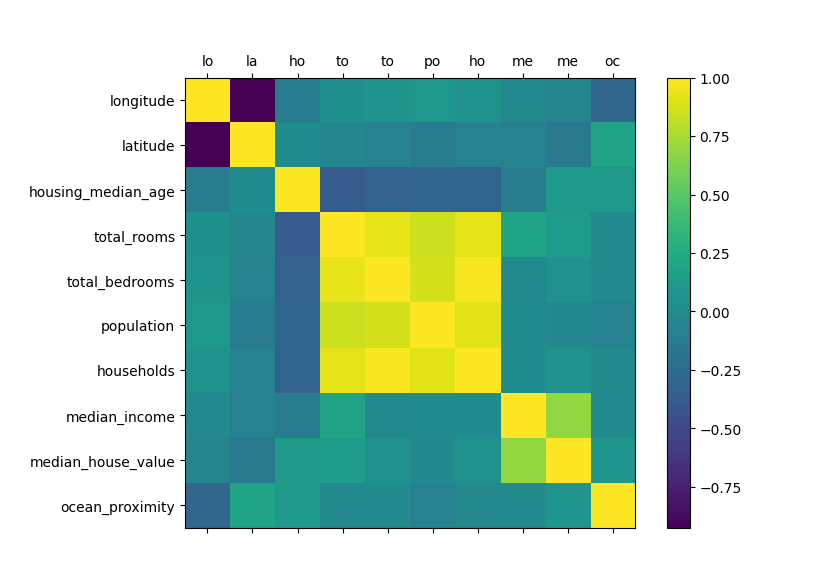
\includegraphics[width=1\linewidth]{figs/correlation.png}
    \caption{Correlation}
    \label{fig:correlation}
\end{figure}

\subsection{Feature distribution}
% List of features

\begin{figure}[htbp]
    \centering
    \begin{minipage}{0.45\textwidth}
        \centering
        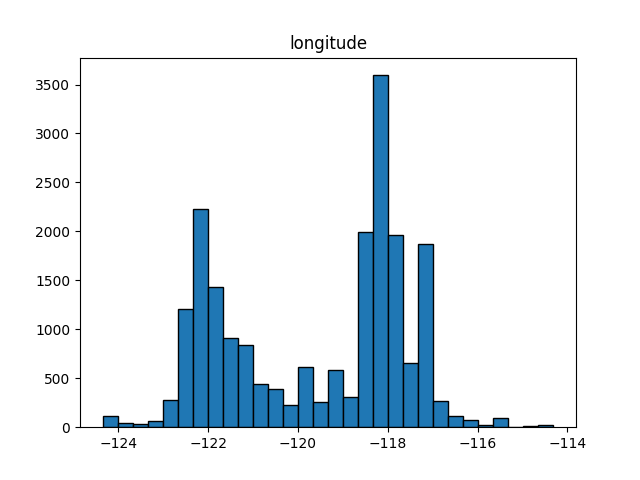
\includegraphics[width=\linewidth]{figs/longitude_distribution.png}
        \caption{Longitude distribution}
        \label{fig:longitude_distribution}
    \end{minipage}\hfill
    \begin{minipage}{0.45\textwidth}
        \centering
        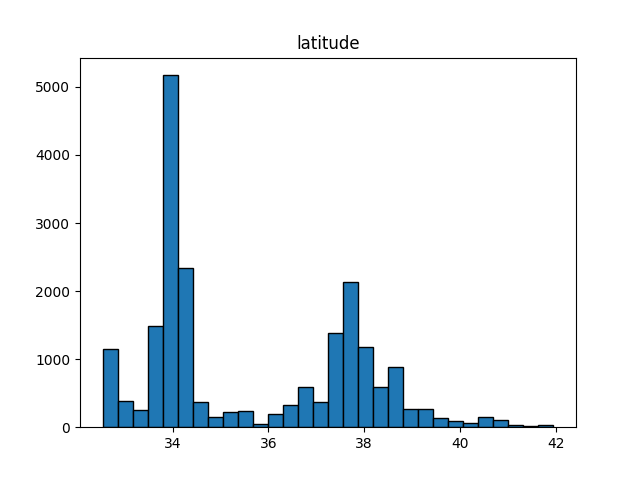
\includegraphics[width=\linewidth]{figs/latitude_distribution.png}
        \caption{Latitude distribution}
        \label{fig:latitude_distribution}
    \end{minipage}
    
    \vspace{0.1cm}  % Adds vertical space between rows
    
    \begin{minipage}{0.45\textwidth}
        \centering
        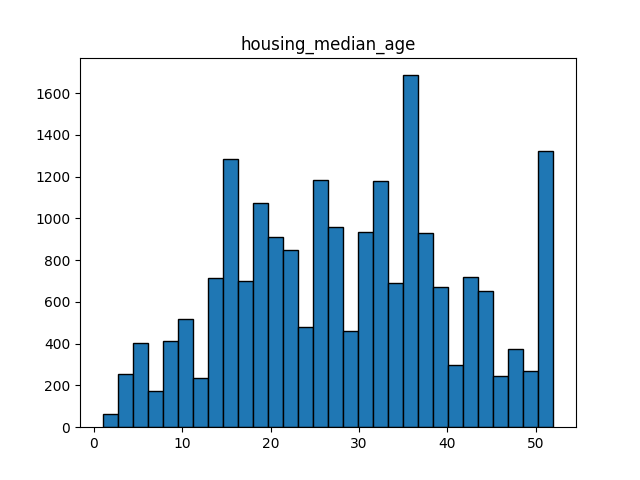
\includegraphics[width=\linewidth]{figs/housing_median_age_distribution.png}
        \caption{Housing median age distribution}
        \label{fig:housing_age_distribution}
    \end{minipage}\hfill
    \begin{minipage}{0.45\textwidth}
        \centering
        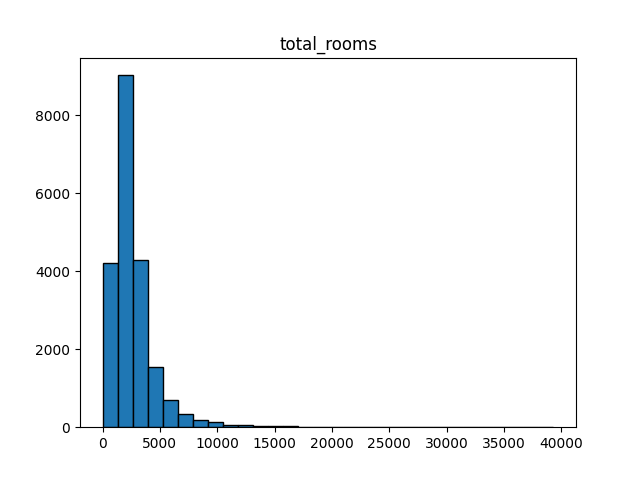
\includegraphics[width=\linewidth]{figs/total_rooms_distribution.png}
        \caption{Total rooms distribution}
        \label{fig:total_rooms_distribution}
    \end{minipage}
    
    \vspace{0.1cm}  % Adds vertical space between rows
    
    \begin{minipage}{0.45\textwidth}
        \centering
        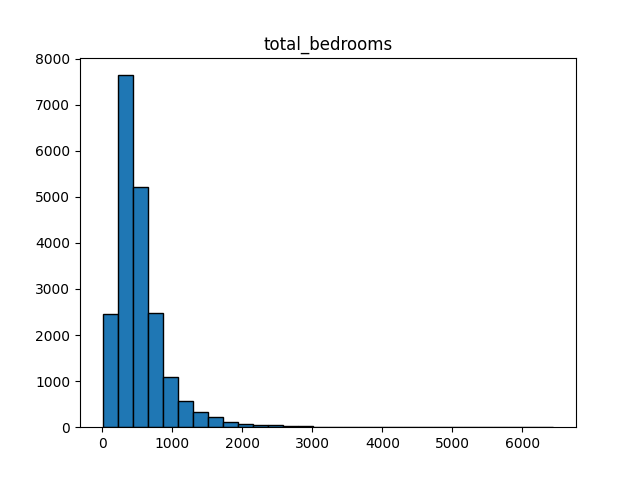
\includegraphics[width=\linewidth]{figs/total_bedrooms_distribution.png}
        \caption{Total bedrooms distribution}
        \label{fig:total_bedrooms_distribution}
    \end{minipage}\hfill
    \begin{minipage}{0.45\textwidth}
        \centering
        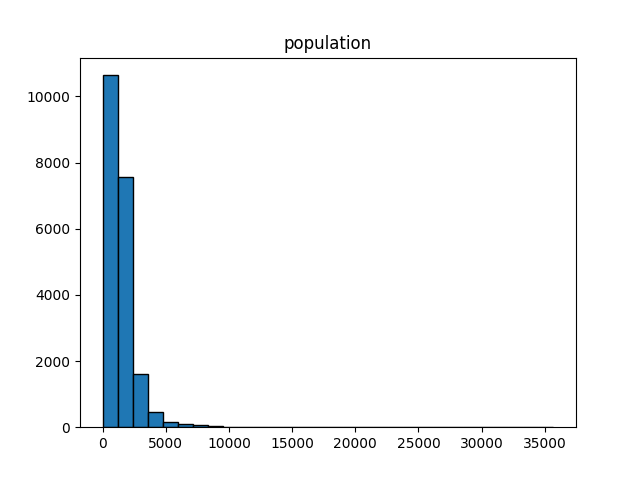
\includegraphics[width=\linewidth]{figs/population_distribution.png}
        \caption{Population distribution}
        \label{fig:population_distribution}
    \end{minipage}
\end{figure}
\begin{figure}[htbp]
    \centering
    \vspace{0.1cm}  % Adds vertical space between rows
    
    \begin{minipage}{0.45\textwidth}
        \centering
        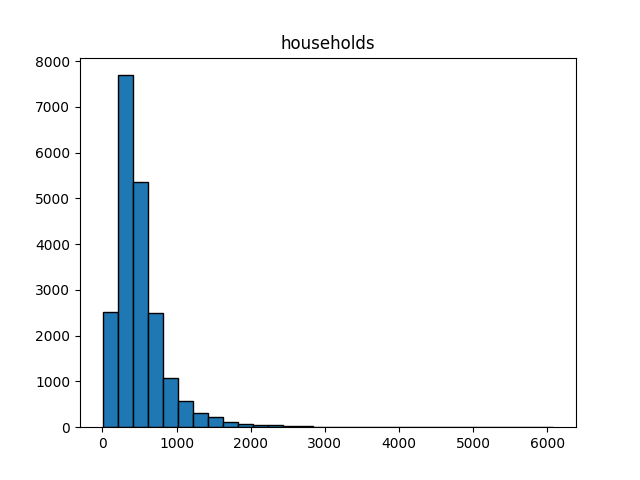
\includegraphics[width=\linewidth]{figs/households_distribution.png}
        \caption{Households distribution}
        \label{fig:households_distribution}
    \end{minipage}\hfill
    \begin{minipage}{0.45\textwidth}
        \centering
        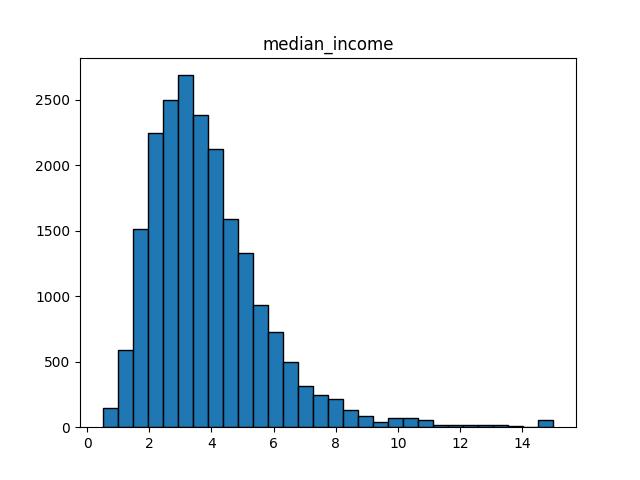
\includegraphics[width=\linewidth]{figs/median_income_distribution.png}
        \caption{Median income distribution}
        \label{fig:median_income_distribution}
    \end{minipage}
    
    \vspace{0.1cm}  % Adds vertical space between rows
    
    \begin{minipage}{0.45\textwidth}
        \centering
        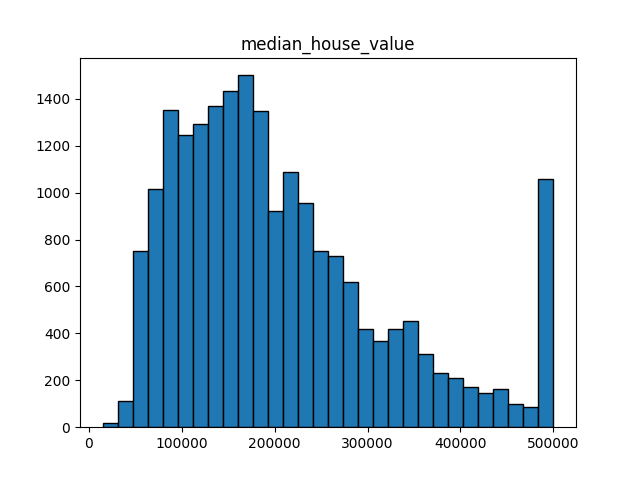
\includegraphics[width=\linewidth]{figs/median_house_value_distribution.png}
        \caption{Median house value distribution}
        \label{fig:median_house_value_distribution}
    \end{minipage}\hfill
    \begin{minipage}{0.45\textwidth}
        \centering
        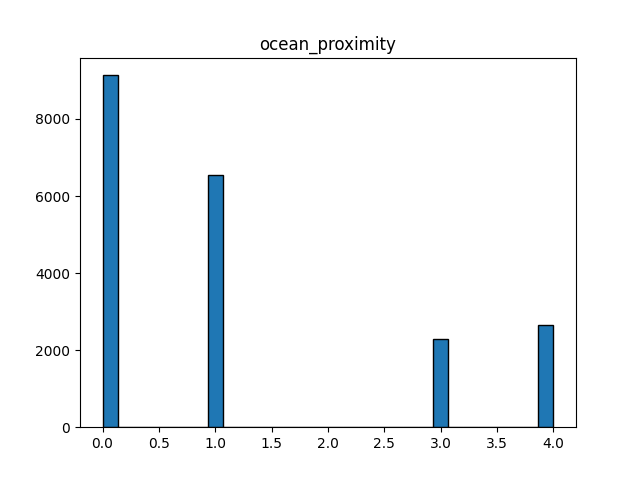
\includegraphics[width=\linewidth]{figs/ocean_proximity_distribution.png}
        \caption{Ocean proximity distribution}
        \label{fig:ocean_proximity_distribution}
    \end{minipage}
\end{figure}


\end{document}
